% Options for packages loaded elsewhere
\PassOptionsToPackage{unicode}{hyperref}
\PassOptionsToPackage{hyphens}{url}
%
\documentclass[landscape, 20pt]{extreport}
%
%\documentclass[
%]{book}
\usepackage{amsmath,amssymb}
\usepackage{lmodern}
\usepackage{iftex}
\ifPDFTeX
  \usepackage[T1]{fontenc}
  \usepackage[utf8]{inputenc}
  \usepackage{textcomp} % provide euro and other symbols
\else % if luatex or xetex
  \usepackage{unicode-math}
  \defaultfontfeatures{Scale=MatchLowercase}
  \defaultfontfeatures[\rmfamily]{Ligatures=TeX,Scale=1}
\fi
% Use upquote if available, for straight quotes in verbatim environments
\IfFileExists{upquote.sty}{\usepackage{upquote}}{}
\IfFileExists{microtype.sty}{% use microtype if available
  \usepackage[]{microtype}
  \UseMicrotypeSet[protrusion]{basicmath} % disable protrusion for tt fonts
}{}
\makeatletter
\@ifundefined{KOMAClassName}{% if non-KOMA class
  \IfFileExists{parskip.sty}{%
    \usepackage{parskip}
  }{% else
    \setlength{\parindent}{0pt}
    \setlength{\parskip}{6pt plus 2pt minus 1pt}}
}{% if KOMA class
  \KOMAoptions{parskip=half}}
\makeatother
\usepackage{xcolor}
\IfFileExists{xurl.sty}{\usepackage{xurl}}{} % add URL line breaks if available
\IfFileExists{bookmark.sty}{\usepackage{bookmark}}{\usepackage{hyperref}}
\hypersetup{
  pdftitle={SCMA329 Practical Mathematical Financial Modeling},
  pdfauthor={Pairote Satiracoo},
  hidelinks,
  pdfcreator={LaTeX via pandoc}}
\urlstyle{same} % disable monospaced font for URLs
\usepackage[margin=1in]{geometry}
\usepackage{longtable,booktabs,array}
\usepackage{calc} % for calculating minipage widths
% Correct order of tables after \paragraph or \subparagraph
\usepackage{etoolbox}
\makeatletter
\patchcmd\longtable{\par}{\if@noskipsec\mbox{}\fi\par}{}{}
\makeatother
% Allow footnotes in longtable head/foot
\IfFileExists{footnotehyper.sty}{\usepackage{footnotehyper}}{\usepackage{footnote}}
\makesavenoteenv{longtable}
\usepackage{graphicx}
\makeatletter
\def\maxwidth{\ifdim\Gin@nat@width>\linewidth\linewidth\else\Gin@nat@width\fi}
\def\maxheight{\ifdim\Gin@nat@height>\textheight\textheight\else\Gin@nat@height\fi}
\makeatother
% Scale images if necessary, so that they will not overflow the page
% margins by default, and it is still possible to overwrite the defaults
% using explicit options in \includegraphics[width, height, ...]{}
\setkeys{Gin}{width=\maxwidth,height=\maxheight,keepaspectratio}
% Set default figure placement to htbp
\makeatletter
\def\fps@figure{htbp}
\makeatother
\setlength{\emergencystretch}{3em} % prevent overfull lines
\providecommand{\tightlist}{%
  \setlength{\itemsep}{0pt}\setlength{\parskip}{0pt}}
\setcounter{secnumdepth}{5}
\usepackage{booktabs}
\usepackage{amsthm}
%\usepackage{LectureNoteMacro}
\usepackage{actuarialangle}
\usepackage{bbm}
\usepackage{mathtools}
\makeatletter
\def\thm@space@setup{%
  \thm@preskip=8pt plus 2pt minus 4pt
  \thm@postskip=\thm@preskip
}
\makeatother
\ifLuaTeX
  \usepackage{selnolig}  % disable illegal ligatures
\fi
\usepackage[]{natbib}
\bibliographystyle{apalike}

\title{SCMA329 Practical Mathematical Financial Modeling}
\author{Pairote Satiracoo}
\date{2021-10-11}

\usepackage{amsthm}
\newtheorem{theorem}{Theorem}[chapter]
\newtheorem{lemma}{Lemma}[chapter]
\newtheorem{corollary}{Corollary}[chapter]
\newtheorem{proposition}{Proposition}[chapter]
\newtheorem{conjecture}{Conjecture}[chapter]
\theoremstyle{definition}
\newtheorem{definition}{Definition}[chapter]
\theoremstyle{definition}
\newtheorem{example}{Example}[chapter]
\theoremstyle{definition}
\newtheorem{exercise}{Exercise}[chapter]
\theoremstyle{definition}
\newtheorem{hypothesis}{Hypothesis}[chapter]
\theoremstyle{remark}
\newtheorem*{remark}{Remark}
\newtheorem*{solution}{Solution}
\begin{document}
\maketitle

\setcounter{chapter}{1}
\hypertarget{bonds-and-inflation}{%
\chapter{Bonds and Inflation}\label{bonds-and-inflation}}



\hypertarget{introduction-to-thai-financial-system}{%
\section{Introduction to Thai Financial
System}\label{introduction-to-thai-financial-system}}

In this chapter, we will first provide an overview of the structure of
the Thai financial system. In the economy, the financial system is of
critical importance. It enables the process of financial intermediation,
which facilitates the movement of money between savers and borrowers and
ensures that money is used effectively to promote economic growth and
development.

According to the document from the Bank of Thailand, a financial system
typically consists of three essential components: financial
institutions, financial markets, and payment system. We shall focus on the first two components.

\begin{enumerate}
\def\labelenumi{\arabic{enumi}.}
\tightlist
\item
  \textbf{Financial Institution}
\end{enumerate}

There are 2 types of financial institution in Thailand, including:

\begin{itemize}
\item \textbf{Depositary Corporations}, for example, commercial banks, Special Financial Institutions (SFIs), Saving Cooperative and credit unions, and money market mutual funds; and
    
\item \textbf{Non-depository corporations}, for example, mutual funds, insurance companies, provident funds, asset management companies, and securities companies.
 
\end{itemize}
\newpage
\begin{enumerate}
\def\labelenumi{\arabic{enumi}.}
\setcounter{enumi}{1}
\tightlist
\item
  \textbf{Financial Markets}
\end{enumerate}

Financial markets provide interaction between those with capital to
invest and those who need capital. Financial markets not only enable
players to raise funds but also to transfer risk (often via derivatives)
and promote commerce.

Financial markets include any place or system that gives buyers and
sellers the ability to trade financial instruments, such as bonds,
shares, different international currencies, and derivatives.

Financial markets include:

\begin{itemize}
    \item \textbf{Money market}
    
The money market is the place for short term financing or borrowing,
which provides short-term liquidity to financial institutions through
interbank lending and repurchase markets. Assets are held in the money
market for a short period of time.

    \item  \textbf{Capital market} 
    
The capital market is the place for long term financing, which
facilitates medium- and long-term capital raising through \textbf{bond and stock
markets}. Assets are held in the capital market for a longer duration
(usually more than a year). It is a risky market and hence it's not
suitable for short term investment .

    \item \textbf{Foreign exchange market}
    

The foreign exchange market is a market for trading and exchanging any
pair of currencies. Foreign exchange rate refers to the value (price) of
one currency in terms of another, such as the exchange rate between the
Thai Baht (THB) and the US Dollar (USD). Demand and supply for the
currencies throughout time determine the fluctuations in the exchange
rate. Such supply and demand are based on market expectations, the value
of global trade, and global money movements.

    \item \textbf{Derivatives market}
    


The derivatives market refers to the financial market for financial
instruments such as futures contracts or options that relate to the
values of their underlying assets.

\end{itemize}

\newpage

\begin{figure}[ht!]
\centering
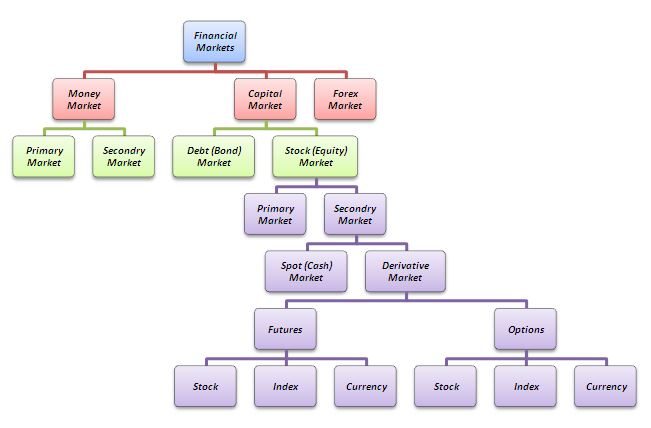
\includegraphics[width=2000mm]{FigFinancialSystem.jpeg}
\caption{Components of Financial markets (image from  \url{https://1.bp.blogspot.com/})}
\end{figure}


\hypertarget{bonds}{%
\section{Bonds}\label{bonds}}

A government or corporation can raise money in the capital markets by
issuing \emph{fixed interest securities (FIS)}, also called \emph{bonds}. Bonds
are a form of medium and long-term securities.

This means that investors will lend money to the issuer (for e.g.~the
government or coporation) and in return will receive fixed interest
payments known as \emph{coupons} at fixed dates plus repayment of the loan at
the end of the term.

\textbf{Note} The loan is usually split into smaller units that can be traded
on a stock exchange. For example, a company raises ฿1,000,000,000 by
issuing 10,000,000 bonds, each one a loan of face value ฿100. These can
be bought and sold on a stock exchange.

\hypertarget{characteristics-of-bonds}{%
\subsection{Characteristics of Bonds}\label{characteristics-of-bonds}}

\begin{enumerate}
\def\labelenumi{\arabic{enumi}.}
\item
  The \emph{nominal amount or face value} of a bond is the amount of the
  loan it represents. The nominal amount is usually ฿1,000 (without
  further specific, we will set the nominal amount to be ฿100.)
\item
  The interest payments are called \emph{coupons}, usually expressed as a
  percentage per year of the nominal amount. The rate of interest
  denoted by \(D\) is also known as \emph{coupon rate}. They are always \textbf{in
  arrears}.
\item
  Coupons are usually expressed as the amount of interest payable in a
  year, but are paid half-yearly (twice per year) or quarterly (4
  times per year)
\item
  \emph{Coupon dates} are the dates on which the bond issuer will make
  interest payments.
\item
  Bonds have \emph{maturity dates} at which point the principal amount must
  be paid back in full.
\item
  The loan is repaid or redeemed at the end of the term. The
  redemption amount per 100 nominal is the \emph{redemption rate}, often
  expressed as a percentage.

  A loan is redeemed

  \begin{itemize}
  \item
    at a premium if redemption rate \textgreater{} 100\%
  \item
    at par if redemption rate = 100\%
  \item
    at a discount if redemption rate \textless{} 100\%
  \end{itemize}
\item
  Many corporate and government bonds are publicly traded; others are
  traded only over-the-counter (OTC) or privately between the borrower
  and lender. (Trading that takes place over-the-counter (OTC), off-exchange takes place directly between two parties without the involvement of an exchange.)
\end{enumerate}

\newpage \begin{example}
\protect\hypertarget{exm:unlabeled-div-46}{}\label{exm:unlabeled-div-46}

\emph{Each bond of ฿100 nominal value carries coupons of 6\%
pa payable half-yearly.}

\end{example}

\textbf{Solution:} The coupon rate of 6\% pa payable half-yearly means that bondholders will receive
\[ \frac{6\%}{2} \times 100 = ฿ 3 \text{ every half-year}.\]

\newpage \begin{example}
\protect\hypertarget{exm:unlabeled-div-47}{}\label{exm:unlabeled-div-47}

\emph{An investor purchases ฿95 for a 5-year fixed interest
bond with face value (or nominal amount of) ฿100. The bond pays coupon
of 6\% pa half-yearly in arrear and the lump sum equal to the nominal
amount in 5 years' time. The cashflows related to the payments of the
bond can be shown as follows:}

\end{example}

\textbf{Solution:} Cashflows are given in the following table.

\begin{longtable}[]{@{}ccccccc@{}}
\toprule
Time (year) & 0 & 0.5 & 1 & 1.5 & \(\ldots\) & 5 \\
\midrule
\endhead
Cashflow & -95 & 3 & 3 & 3 & \(\ldots\) & \(3 + 100\) \\
\bottomrule
\end{longtable}

Examples of bonds include

\begin{itemize}
\item
  domestic bonds issued in the domestic currency such as gilts issued
  by UK government and treasury bonds issued by US government.
\item
  Eurobonds where an issuer sells the bond outside the domestic
  country.
\item
  debenture bonds issued by corporations.
\end{itemize}

\newpage \begin{example}
\protect\hypertarget{exm:exampleBondPrice}{}\label{exm:exampleBondPrice}

\emph{A company issues a 10-year bond, to be redeemed at
102\%, with coupon of 6\% pa payable half-yearly in arrears. The nominal
amount of each bond is ฿100. What repayments are made?}

\end{example}

\textbf{Solution:} Cashflows are given in the following table.

\begin{longtable}[]{@{}cccccccc@{}}
\toprule
Time (year) & 0 & 0.5 & 1 & 1.5 & \(\ldots\) & 9.5 & 10 \\
\midrule
\endhead
Cashflow & \(P\) & 3 & 3 & 3 & \(\ldots\) & \(3\) & \(3 + 102\) \\
\bottomrule
\end{longtable}

Here the bond price in the table above is denoted by \(P\).

The following questions may be asked:

\begin{itemize}
\item
  At what price should be paid by an investor to obtain a net yield of
  \(i\) per annum?
\item
  Given the price of the fixed interest bond, what is the net yield
  per annum will be obtained?
\end{itemize}

\hypertarget{bond-prices}{%
\subsection{Bond prices}\label{bond-prices}}

Given a yield \(i\%\), the price of a bond can be computed by discounting
all the future payments received net of any tax.

\newpage \begin{example}
\protect\hypertarget{exm:exampleBondPrice2}{}\label{exm:exampleBondPrice2}

\emph{A tax-exempt investor buy the bond in Example \ref{exm:exampleBondPrice} on its issue date. Calculate the price the
investor should pay to obtain a yield of 9\%.}

\end{example}

\textbf{Solution:}
Appplying the Principle of Equivalence: by equate the present value of the future incomes at 9\% with the unknown price \(P\).

\[P = \frac{6}{2} a^j_{\angl{20}} + 102 (\frac{1}{1.09})^{20},\]
where \(j = (1.09)^{(1/2)} - 1 = 0.044031.\)
This gives \(P = 82.44\). It should be emphasised that the price in this example differs from the nominal amount of 100.

\newpage \begin{example}
\protect\hypertarget{exm:unlabeled-div-48}{}\label{exm:unlabeled-div-48}

\emph{Refer to Examples
\ref{exm:exampleBondPrice} and
\ref{exm:exampleBondPrice2}. After the 10th coupon has been paid, the
investor sells the bond. At that time the market yield on comparable
5-year bonds is 7\% pa effective.}

\begin{enumerate}
\def\labelenumi{\arabic{enumi}.}
\item
  \emph{Calculate the price that he will obtain.}
\item
  \emph{Calculate the yield that the first investor obtains if he paid
  ฿82.44 and received 10 coupon payments of ฿3 each and sold the bond
  after 5 years at the price of ฿97.75.}
\end{enumerate}

\end{example}

\textbf{Solution:}

\begin{enumerate}
\def\labelenumi{\arabic{enumi}.}
\tightlist
\item
  The remaining payments are shown in the table below.
\end{enumerate}

\begin{longtable}[]{@{}cccccccc@{}}
\toprule
Time (half-year) & 10 & 11 & 12 & 13 & \(\ldots\) & 19 & 20 \\
\midrule
\endhead
Cashflow & \(-\) & 3 & 3 & 3 & \(\ldots\) & \(3\) & \(3 + 102\) \\
\bottomrule
\end{longtable}

Working in unit of half-year, we first calculate the effective rate per half-year, denoted by \(k\), that is equivalent to \(i = 7\%\).

\[ k = (1.07)^{(1/2)} - 1 = 0.034408. \]

The price \(P'\) that he will obtain follows from the following equation.
\[P' = 3 a^k_{\angl{10}} + 102 (\frac{1}{1.07})^{5} = 97.75.\]

\begin{enumerate}
\def\labelenumi{\arabic{enumi}.}
\setcounter{enumi}{1}
\tightlist
\item
  The payments of the investor are shown in the table below.
\end{enumerate}

\begin{longtable}[]{@{}cccccccc@{}}
\toprule
Time (half-year) & 0 & 1 & 2 & 3 & \(\ldots\) & 9 & 10 \\
\midrule
\endhead
Cashflow & -82.44 & 3 & 3 & 3 & \(\ldots\) & \(3\) & \(3 + 97.75\) \\
\bottomrule
\end{longtable}

Let \(i\) denote the yield (per half-year) that the first investor obtains.
Working at time 10, the equation of value of the cashflows is
\[ f(i) = 82.44 (1+i)^{10} - 3 s^i_{\angl{10}} - 97.75 = 0.\]
By linear interpolation, we have
\[ f(0.05) = -1.1976, \quad f(0.06) = 10.3451, \]
and hence, the approximate of \(i\) is \(i^* \approx 0.051038\). The annual yield is then approximately equal to \((1 + 0.051038)^2 - 1 = 10.468\%\)

\textbf{Notes}

\begin{enumerate}
\def\labelenumi{\arabic{enumi}.}
\item
  If the investor is not subject to taxation, the yield is called the
  \emph{gross yield}.
\item
  The yield obtained by holding the bond until redemption is called
  \emph{redemption yield}. This is quoted in financial newspapers.
\item
  If a bond is sold before redemption, the yield that the investor
  obtains is called \emph{realised yield}. This yield depends on both the
  buying and selling prices.
\end{enumerate}

\textbf{Notes}

\begin{enumerate}
\def\labelenumi{\arabic{enumi}.}
\item
  There is an inverse relationship between the bond prices and yields.
\item
  The nominal amount of the loan is just a theoretical figure on which
  the coupon and redemption rates are based.
\item
  The amount of capital the borrower can actually raise on the issue
  date is the price that investors are willing to pay for the future
  income stream and also set by supply and demand.
\item
  The investors also consider the \textbf{credit risk} of the borrower. It
  is the risk that they might default on interest and capital
  payments.
\item
  The greater the credit risk, the higher the yield they will require.
\item
  The bonds can be traded on an exchange at any time until it is
  redeemed. The prices will depend on the remaining term to redemption
  and market conditions such as the yields obtainable on other
  investments.
\end{enumerate}

\hypertarget{no-tax}{%
\subsection{No tax}\label{no-tax}}

A tax-exempt investor receives the full amount of the coupon and
redemption payments. The price of an \(n\) year fixed interest bond which
pays coupons of \(D\) per annum payable \(p\) thly in arrear and has
redemption amount \(R\) is \[P = D a_{\angln}^{(p)} + R v^n\] at rate \(i\)
per annum.

In practice, we can calculate by using a suitable time period, for
example a period of half a year as shown in the previous examples. Then
the formula can be written as
\[P = \frac{D}{2} a_{\angl{2n}} + R v^{2n}\]

\hypertarget{income-tax}{%
\subsection{Income tax}\label{income-tax}}

Suppose an investor is subject to income tax at rate \(t_1\) on the
coupons, which is due at the time that the coupons are paid. Tax will
affect both yields and bond prices. In general, the price of this bond,
an \(n\) year fixed interest bond which pays coupons of \(D\) per annum
payable \(p\) thly in arrear and has redemption amount \(R\) is
\[P = (1 - t_1) D a_{\angln}^{(p)} + R v^n\] at rate \(i\) per annum. Here
the rate is called the \emph{net yield}.

\newpage \begin{example}
\protect\hypertarget{exm:unlabeled-div-49}{}\label{exm:unlabeled-div-49}

\emph{An investor liable to income tax at 30\% buys a 15-year
fixed interest bond which is redeemable at par and pays coupons of 8\% pa
half-yearly in arrear. Calculate the price the investor should pay to
obtain a net yield of 9\% pa.}

\end{example}

\textbf{Solution:} Coupon payments after tax are
\[ (1 - t_1) D = (1 - 0.3) \frac{8\%}{2} \times 100 = 2.8.\]

The payments of the investor are shown in the table below.

\begin{longtable}[]{@{}cccccccc@{}}
\toprule
Time (half-year) & 0 & 1 & 2 & 3 & \(\ldots\) & 29 & 30 \\
\midrule
\endhead
Cashflow & \(P\) & 2.8 & 2.8 & 2.8 & \(\ldots\) & 2.8 & \(2.8 + 100\) \\
\bottomrule
\end{longtable}

The price the investor should pay to obtain a net yield of 9\% pa can be calculated from
\[P = 2.8 a^j_{\angl{30}} + 100 (\frac{1}{1+j})^{30} = 73.59,\]
where where \(j = (1.09)^{(1/2)} - 1 = 0.044031\) per half-year effective.

\hypertarget{capital-gains-tax-cgt}{%
\subsection{Capital gains tax (CGT)}\label{capital-gains-tax-cgt}}

Capital gains tax is a tax levied on the capital gain made on the
redemption of a bond (or the sale of the bond if sold earlier). The
capital gain is simply the difference between

Note that \textbf{capital gain} refers to an increase in a capital asset's value and is considered to be realized when the asset is sold. A \textbf{capital loss} is incurred when there is a decrease in the capital asset value compared to an asset's purchase price.

\newpage \begin{example}
\protect\hypertarget{exm:unlabeled-div-50}{}\label{exm:unlabeled-div-50}

\emph{An investor liable to the capital gains tax at 20\%
purchases two bonds}

\begin{itemize}
\item
  \emph{Bond A for the price of ฿102 and}
\item
  \emph{Bond B for the price of ฿98.}
\end{itemize}

\emph{Calculate the capital gains tax on each bond if the investor sells them
both one year later for ฿100 each.}

\end{example}

\textbf{Solution:}

\begin{itemize}
\item
  Bond A: Tax payment is \(0.2 \times \max\{100 - 102,0 \} = 0\) (i.e.~capital loss)
\item
  Bond B: Tax payment is \(0.2 \times \max\{100 - 98,0 \} = 0.4\) (i.e.~capital gain)
\end{itemize}

Here we assume that no `relief', i.e.~we cannot add the two bonds together and say we bought the two bonds for ฿200 and sold the bonds for ฿200.

\textbf{Notes}

\begin{enumerate}
\def\labelenumi{\arabic{enumi}.}
\item
  Similar to income tax, the price of the bond is then calculated on
  the net redemption received after tax has been deducted.
\item
  When the purchase and sale (or redemption) prices are known, it it
  easy to calculate the yield.
\item
  In contrast, as the price depends on whether there is a capital gain
  and the capital gain depends on the price, it is not easy to
  calculate the price for a given redemption yield. There is a test to
  determine whether CGT is payable.
\end{enumerate}

\newpage \begin{example}
\protect\hypertarget{exm:unlabeled-div-51}{}\label{exm:unlabeled-div-51}

\emph{An investor liable to the capital gains tax at 20\%
purchases a 10-year bond with an annual coupon of 8\% pa payable yearly
in arrear, to be redeemed at par.}

\begin{enumerate}
\def\labelenumi{\arabic{enumi}.}
\item
  \emph{Calculate the redemption yield the investor obtain if the price is
  ฿96 per ฿100 nominal.}
\item
  \emph{What price should the investor pay to obtain a yield of 7\% pa
  effective?} (see note below)
\item
  \emph{What price should the investor pay to obtain a yield of 9\% pa effective?}\\
\end{enumerate}

\end{example}

\textbf{Note} In this example, we can guess whether CGT is payable because we have calculated the price to yield 8.546\% from the above question. Then we can use the appropriate equation to calculate the bond price and check whether or not our initial guess was correct.

\hypertarget{inflation}{%
\section{Inflation}\label{inflation}}

Inflation is a measure of the rate of change in the price of consumer
goods and services, such as food and beverages, transportation and
housing.

\begin{itemize}
\item
  In Thailand or US, it is measured with reference to a \textbf{consumer
  price index} (or CPI). In UK, it is measured in terms of \textbf{retail
  price index} (RPI).
\item
  Bureau of Trade and Economic Indices reports the CPI on a monthly
  basis.
\item
  High inflation means that prices increase quickly and hence \textbf{the
  purchasing power} significantly decreases.
\end{itemize}

Let \(Q(t)\) be the CPI at time \(t\). Then the rate of inflation per year
denoted by \(q(t)\) is \[q(t) = \frac{Q(t)}{Q(t-1)} - 1.\] The average
inflation rate per year between time \(s\) and \(t\), denoted by \(\bar{q}\),
satisfies \[(1 + \bar{q})^{t-s} = \frac{Q(t)}{Q(s)},\] and hence
\[\bar{q} = \left( \frac{Q(t)}{Q(s)}  \right)^{1/(t-s)} - 1.\]

\newpage \begin{example}
\protect\hypertarget{exm:unlabeled-div-52}{}\label{exm:unlabeled-div-52}

\emph{A set of goods costs ฿98.25 in January 2013 and
฿101.44 in January 2018. Calculate the average inflation rate \(\bar{q}\)
over this period.}

\end{example}

\textbf{Solution:} The increase from Jan 2013 to Jan 2018 (5 years) is
\[\frac{101.44}{98.25}  - 1 =   0.032.\] The average of inflation rate
\(\bar{q}\) is given by \[(1  + \bar{q})^5 = 1.032.\] Therefore
\(\bar{q} = 0.64\%\).

Therefore, ฿1 in January 2013 buys as much as ฿1.032 in January 2018.

The following table shows the monthly consumer price indices from
January 2011 to December 2019. Source:
\url{http://www.price.moc.go.th/}

\begin{longtable}[]{@{}
  >{\raggedright\arraybackslash}p{(\columnwidth - 24\tabcolsep) * \real{0.08}}
  >{\raggedright\arraybackslash}p{(\columnwidth - 24\tabcolsep) * \real{0.08}}
  >{\raggedright\arraybackslash}p{(\columnwidth - 24\tabcolsep) * \real{0.08}}
  >{\raggedright\arraybackslash}p{(\columnwidth - 24\tabcolsep) * \real{0.08}}
  >{\raggedright\arraybackslash}p{(\columnwidth - 24\tabcolsep) * \real{0.08}}
  >{\raggedright\arraybackslash}p{(\columnwidth - 24\tabcolsep) * \real{0.08}}
  >{\raggedright\arraybackslash}p{(\columnwidth - 24\tabcolsep) * \real{0.08}}
  >{\raggedright\arraybackslash}p{(\columnwidth - 24\tabcolsep) * \real{0.08}}
  >{\raggedright\arraybackslash}p{(\columnwidth - 24\tabcolsep) * \real{0.08}}
  >{\raggedright\arraybackslash}p{(\columnwidth - 24\tabcolsep) * \real{0.08}}
  >{\raggedright\arraybackslash}p{(\columnwidth - 24\tabcolsep) * \real{0.08}}
  >{\raggedright\arraybackslash}p{(\columnwidth - 24\tabcolsep) * \real{0.08}}
  >{\raggedright\arraybackslash}p{(\columnwidth - 24\tabcolsep) * \real{0.08}}@{}}
\caption{\label{tab:tableCPI} The monthly consumer price indices from
January 2011 to December 2019.}\tabularnewline
\toprule
\begin{minipage}[b]{\linewidth}\raggedright
Year
\end{minipage} & \begin{minipage}[b]{\linewidth}\raggedright
1
\end{minipage} & \begin{minipage}[b]{\linewidth}\raggedright
2
\end{minipage} & \begin{minipage}[b]{\linewidth}\raggedright
3
\end{minipage} & \begin{minipage}[b]{\linewidth}\raggedright
4
\end{minipage} & \begin{minipage}[b]{\linewidth}\raggedright
5
\end{minipage} & \begin{minipage}[b]{\linewidth}\raggedright
6
\end{minipage} & \begin{minipage}[b]{\linewidth}\raggedright
7
\end{minipage} & \begin{minipage}[b]{\linewidth}\raggedright
8
\end{minipage} & \begin{minipage}[b]{\linewidth}\raggedright
9
\end{minipage} & \begin{minipage}[b]{\linewidth}\raggedright
10
\end{minipage} & \begin{minipage}[b]{\linewidth}\raggedright
11
\end{minipage} & \begin{minipage}[b]{\linewidth}\raggedright
12
\end{minipage} \\
\midrule
\endfirsthead
\toprule
\begin{minipage}[b]{\linewidth}\raggedright
Year
\end{minipage} & \begin{minipage}[b]{\linewidth}\raggedright
1
\end{minipage} & \begin{minipage}[b]{\linewidth}\raggedright
2
\end{minipage} & \begin{minipage}[b]{\linewidth}\raggedright
3
\end{minipage} & \begin{minipage}[b]{\linewidth}\raggedright
4
\end{minipage} & \begin{minipage}[b]{\linewidth}\raggedright
5
\end{minipage} & \begin{minipage}[b]{\linewidth}\raggedright
6
\end{minipage} & \begin{minipage}[b]{\linewidth}\raggedright
7
\end{minipage} & \begin{minipage}[b]{\linewidth}\raggedright
8
\end{minipage} & \begin{minipage}[b]{\linewidth}\raggedright
9
\end{minipage} & \begin{minipage}[b]{\linewidth}\raggedright
10
\end{minipage} & \begin{minipage}[b]{\linewidth}\raggedright
11
\end{minipage} & \begin{minipage}[b]{\linewidth}\raggedright
12
\end{minipage} \\
\midrule
\endhead
2011 & 91.93 & 92.3 & 92.75 & 94.03 & 94.35 & 94.47 & 94.64 & 95.05 & 94.73 & 94.91 & 95.12 & 94.66 \\
2012 & 95.03 & 95.38 & 95.95 & 96.35 & 96.73 & 96.89 & 97.22 & 97.61 & 97.93 & 98.06 & 97.71 & 98.09 \\
2013 & 98.25 & 98.46 & 98.52 & 98.68 & 98.92 & 99.07 & 99.17 & 99.16 & 99.32 & 99.49 & 99.59 & 99.73 \\
2014 & 100.15 & 100.39 & 100.6 & 101.1 & 101.51 & 101.4 & 101.32 & 101.23 & 101.06 & 100.96 & 100.84 & 100.33 \\
2015 & 99.74 & 99.86 & 100.03 & 100.05 & 100.22 & 100.32 & 100.25 & 100.03 & 99.98 & 100.18 & 99.86 & 99.47 \\
2016 & 99.21 & 99.36 & 99.57 & 100.11 & 100.68 & 100.71 & 100.36 & 100.32 & 100.36 & 100.52 & 100.46 & 100.59 \\
2017 & 100.75 & 100.79 & 100.33 & 100.49 & 100.64 & 100.66 & 100.53 & 100.64 & 101.22 & 101.38 & 101.45 & 101.37 \\
2018 & 101.44 & 101.21 & 101.12 & 101.57 & 102.14 & 102.05 & 102.00 & 102.27 & 102.57 & 102.63 & 102.40 & 101.73 \\
2019 & 101.71 & 101.95 & 102.37 & 102.82 & 103.31 & 102.94 & 103.00 & 102.80 & 102.90 & 102.74 & 102.61 & 102.62 \\
\bottomrule
\end{longtable}

Figure \ref{fig:figCPI} shows the monthly consumer price indices from January 2011
to December 2019.

\begin{figure}

{\centering 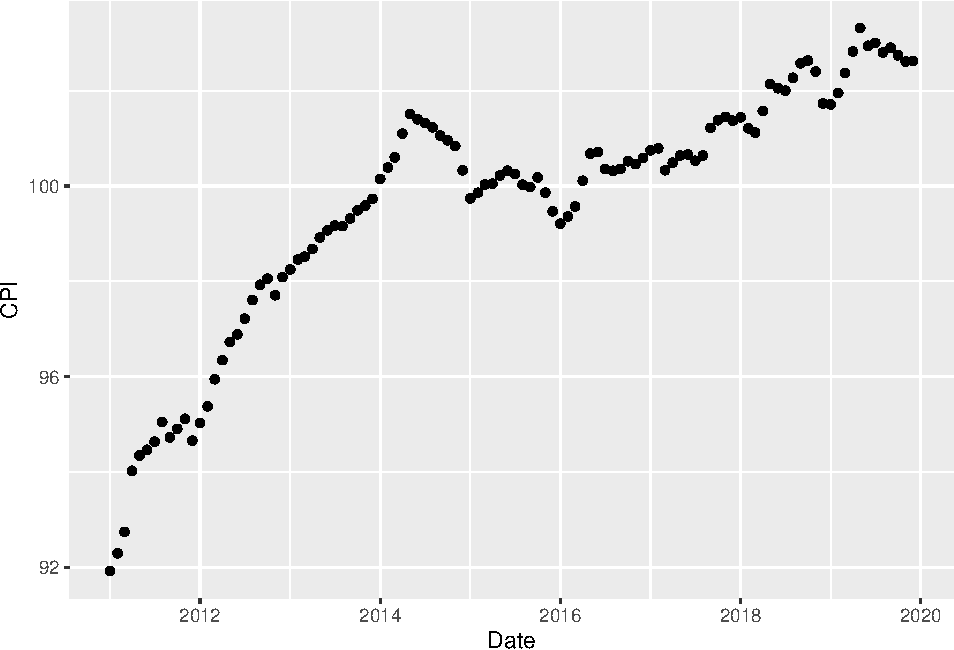
\includegraphics{figCPI-1} 

}

\caption{The monthly consumer price indices from January 2011 to December 2019}\label{fig:figCPI}
\end{figure}

\begin{figure}
\centering
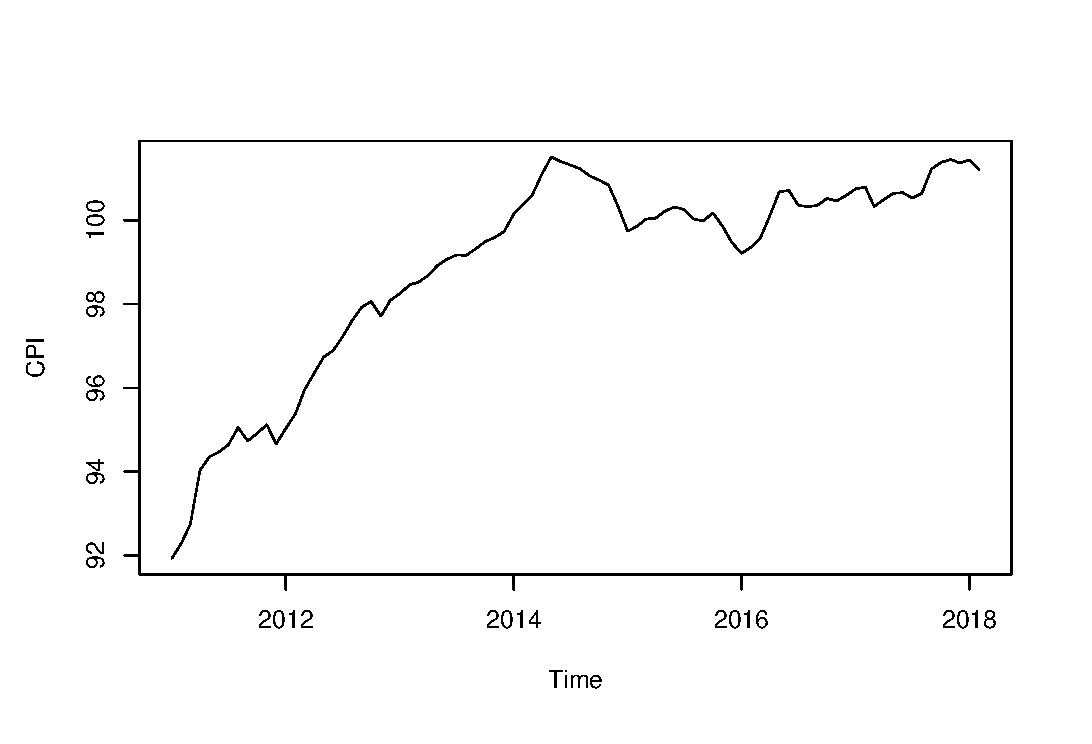
\includegraphics{CPIGraph.eps}
\caption{image}
\end{figure}

\newpage \begin{example}
\protect\hypertarget{exm:unlabeled-div-53}{}\label{exm:unlabeled-div-53}

\emph{An investment contract made on January 2018 promises
to pay an investor of ฿10,000 in 5 years' time. Assume the average
inflation rate at \(\bar{q} = 0.64\%\) for the next 5 years.}

\emph{If a bowl of noodles costs ฿100 in 2018, then ฿10,000 could buy 100
bowls. How many bowls of noodles would the payment of ฿10,000 buy in the
next 5 years?}

\emph{\textbf{Solution:} In Jan 2018, ฿100 buys as much as \(100 (1.0064)^5 =\)
฿103.2 in Jan 2023.}

\emph{So ฿10000 in Jan 2023 could buy
\[\frac{10000}{103.2} \approx 96 \text{ bowls}.\] Notice that we divide
by \((1 + \bar{q})^5\) to calculate how much your money is worth at the
end of the next five years.}

\begin{itemize}
\item
  \emph{The quantity of goods that can be bought with 10,000 in January
  2023 reduces from 100 to 96 bowls.}
\item
  \emph{The effect of inflation results in the reduction of the purchasing
  power of a unit of money in January 2023 compared to that in
  January 2018.}
\item
  \emph{The amount of ฿10,000 is referred to as the \textbf{monetary} (or
  \textbf{nominal}) payment in 5 years. This is the amount of money that
  change hands.}
\item
  \emph{The \textbf{real payment of ฿10,000 (due at time 5 years) in time 0
  unit} is \[\begin{aligned}
  10000 \frac{Q(0)}{Q(5)} &=  10000  \frac{1}{(1.0064)^5} \\
                           &=  9686.05.\end{aligned}\] Here we have
  less purchasing power with your money at the end of the five years
  than you had at the start of the year.}
\item
  \emph{The real payment (in time 0) is the purchase power of 10,000 paid
  in 5 years relative to today. \textbf{It is the amount of cash in hand at
  the end of the period reduced for the effects of inflation}.}
\item
  \emph{In general, ฿X at time \(t\) has the purchasing power relative to
  time \(s\) of \[X \cdot \frac{Q(s)}{Q(t)}.\]}
\end{itemize}

\end{example}

\hypertarget{real-rates-of-interest}{%
\subsection{Real rates of interest}\label{real-rates-of-interest}}

The rate of interest which is calculated using monetary payments is
called a \textbf{money (or monetary or nominal) rate of interest}.

The \textbf{real rate of interest} is calculated using real payments.

\newpage \begin{example}
\protect\hypertarget{exm:unlabeled-div-54}{}\label{exm:unlabeled-div-54}

\emph{An investor deposits 100 at time 0 and receives 120
after one year.}

\begin{itemize}
\item
  \emph{The monetary rate of interest effective is
  \[\frac{120}{100} - 1 = 20\%.\]}
\item
  \emph{Suppose that the inflation rate over this one year period is 4\%.
  Calculate the real payment of 120 at time 1 and the real rate of
  interest. After adjusting for the inflation rate, the real rate of
  interest can be calculated by first expressing both payments in
  units of the same purchasing power.}

  \begin{itemize}
  \item
    \emph{In term of time 0 money unit, the transaction is represented
    by}

    \emph{Here, the real payment of 120 due in 1 year in terms of time 0
    unit is \(\displaystyle{120 \cdot \frac{1}{1.04} = 115.38}\).
    Hence the real rate of interest is 15.38\%.}
  \item
    \emph{In term of time 1 money unit, the transaction is represented
    by}

    \emph{Similarly, we instead calculate the real payment of 100
    relative to time 1, which gives \(100 \cdot 1.04 = 104\). The real
    rate of interest is \[\frac{120}{104} - 1 = 15.38\%,\] which is
    the same as the previous case.}
  \end{itemize}
\end{itemize}

\end{example}

\hypertarget{real-yields}{%
\subsection{Real yields}\label{real-yields}}

It is often useful to look at the rate of return earned on an investment
after taking into account of inflation. As analogous to the real rate of
interest, a \textbf{real yield} is calculated using real payments, which can
be obtained by expressing payments in units of the same purchasing power
\textbf{at some specific date}.

\newpage \begin{example}
\protect\hypertarget{exm:unlabeled-div-55}{}\label{exm:unlabeled-div-55}

\emph{A 5-year bond with nominal value of ฿100 was issued
in January 2013. The coupon rate was 8\% p.a. payable yearly in arrears.
Redemption was at par after 5 years. The bond was issued at 100\%.
Calculate the yield to a non-tax paying investor}

\begin{enumerate}
\def\labelenumi{\arabic{enumi}.}
\item
  \emph{in monetary terms \textbf{Solution:}}

  \emph{The transaction together with the inflation indices \(Q(t)\) at time
  \(t\) is shown as follows:}

  \emph{Clearly, the monetary rate of return on this transaction is 8\%.
  This is because the investor receives the interest payment of ฿8 at
  the end of each year plus the initial capital of ฿100 at the end of
  five years.}

  \emph{Alternatively, one can solve for the monetary rate of return from
  the following equation of value
  \[f(i) = -100 + 8 a^i_{\actuarialangle{5}} + 100\frac{1}{(1+i)^5} = 0.\]}
\item
  \emph{in real terms with reference to the CPI.}

  \emph{Taking into account of the inflation rates, we calculate the real
  payment in term of time 0 unit by dividing the monetary amounts by
  the \textbf{proportional} increase in the inflation index from 0 to \(t\).}

  \emph{The real yield \(i'\) p.a. effective solve the equation of value as
  follows:
  \[f(i') = -100 + 7.85 v  + 7.88v^2 + 7.91v^3 + 7.80v^6 + 104.6v^5 = 0,\]
  which gives \(i' \approx 7.30\%\) by the linear interpolation.}
\end{enumerate}

\end{example}

In general, the real yield \(i'\) for a series of cashflows
\(C(t_1), C(t_2), \ldots, C(t_n)\), given associated inflation index
\(Q(t_k)\) for \(k = 1, \ldots, n\), can be obtained in terms of time 0
money units as
\[\sum_{k=1}^n C(t_k) \frac{Q(0)}{Q(t_k)} \frac{1}{(1 + i')^{t_k}} = 0.\]
This is equivalent to
\[\sum_{k=1}^n C(t_k) \frac{1}{Q(t_k)} \frac{1}{(1 + i')^{t_k}} = 0.\]
Therefore, \textbf{the real yield is independent of the date the payment units
are adjusted to}.

\hypertarget{calculating-real-yields-given-constant-inflation-assumptions}{%
\subsection{Calculating real yields given constant inflation assumptions}\label{calculating-real-yields-given-constant-inflation-assumptions}}

For future cashflows, the inflation index will not be known. Suppose we
assume a constant rate of inflation \(q\) p.a. The cashflows \(C(t_k)\) at
time \(t_k\) have the purchasing power at time 0 (or real payments
relative to time 0) \[\begin{aligned}
    C(t_k) \cdot \frac{Q(0)}{Q(t_k)} &=     C(t_k) \cdot \frac{Q(0)}{Q(0)(1+q)^{t_k}}  =  C(t_k) \cdot \frac{1}{(1+q)^{t_k}} , \quad k = 1, \ldots, n.\end{aligned}\]
The relation between the real yield \(i'\), the constant rate of inflation
\(q\) and the monetary yield \(i\) can be obtained as follows: From the
equation of value, \[\begin{aligned}
    0   &= \sum_{k=1}^n C(t_k) \frac{Q(0)}{Q(t_k)} \frac{1}{(1 + i')^{t_k}} \\
        &=  \sum_{k=1}^n C(t_k)  \cdot \frac{1}{(1+q)^{t_k}}\cdot \frac{1}{(1 + i')^{t_k}}\end{aligned}\]
With no inflation adjustment, the monetary rate of return \(i\) satisfies
\[0 =  \sum_{k=1}^n C(t_k)  \cdot \frac{1}{(1+i)^{t_k}}.\] Therefore, if
\textbf{we assume a constant rate of inflation} \(q\) p.a., then the following
relation holds: \[(1 +i) = ( 1 + q)(1+i').\] This provides the
relationship between the real yield \(i'\), the monetary yield \(i\) and the
inflation rate \(q\).

\hypertarget{index-linked-securities}{%
\subsection{Index-linked securities}\label{index-linked-securities}}

An index-linked security is an investment security in which interest
payments and the redemption are adjusted in line with inflation index
values by linking the payments to the Consumer Price Index (CPI). The
reasons for these types of security are

\begin{itemize}
\item
  to protect investors against inflation risk, and
\item
  to help pension funds to provide index-link benefits so that the
  index-link liability can be matched with the index-link asset.
\end{itemize}

\newpage \begin{example}
\protect\hypertarget{exm:unlabeled-div-56}{}\label{exm:unlabeled-div-56}

\emph{Consider an index-link bond of a nominal of ฿100
issued at time \(t_0\), bearing an annual coupon of \(C\%\) payable \(m\)
times a year and a redemption is at \(R\%\). Then per ฿100 nominal, the
monetary amount (actual cashflow) of an interest payment \(D(t_k)\) at
time \(t_k\) is}

\emph{The monetary amount of the redemption amount at time \(t_n\) is}

\end{example}

\newpage \begin{example}
\protect\hypertarget{exm:exampleILB}{}\label{exm:exampleILB}

\emph{An investor purchased a 3-year index-linked bond in
January 2015. The investor received payments at the end of each year
plus a final redemption amount, all of which were adjusted in line with
the CPI values reported in Table \ref{tab:tableCPI}.
Calculate the actual payments received by the investor.}

\end{example}

\textbf{Note} In practice, due to delays in calculating the index, the
payments (or cashflows) will be adjusted based on the inflation index
value from an earlier period.

Let \(s\) denote the indexation time lag. The payments are adjusted with
reference to inflation index value at time \(s\) (months) before the
payment is made. Then the monetary amount of an interest payment
\(D(t_k)\) per ฿100 nominal at time \(t_k\) is
\[\displaystyle D(t_k) = 100 \frac{C}{m} \cdot \frac{Q(t_k - \frac{s}{12})}{Q(t_0 - \frac{s}{12})}\]
and the monetary amount of redemption at time \(t_n\) is
\[D(t_n) = 100 R \cdot \frac{Q(t_n - \frac{s}{12})}{Q(t_0 - \frac{s}{12})}.\]
The term \(Q(t_0 - \frac{s}{12})\) is called the base inflation figure
(the base CPI figure).

\newpage \begin{example}
\protect\hypertarget{exm:unlabeled-div-57}{}\label{exm:unlabeled-div-57}

\emph{Repeat Example\ref{exm:exampleILB}
for a 3-year index linked bond. The indexation adjustments are made
according to the CPI three months before each payment, i.e.~\(s = 3\)
months.}

\end{example}

\newpage \begin{example}
\protect\hypertarget{exm:exampleILB2}{}\label{exm:exampleILB2}

\emph{In January 2015, the government issued an
index-linked bond of term 10 years. Coupons are payable half-yearly in
arrears, and the annual nominal coupon rate is 4\%. The coupons and
redemption amount are adjusted with reference to the inflation index
value 3 months before the payment is made.}

\emph{Assume the constant inflation rate from February 2018 is 2\% p.a.}

\begin{enumerate}
\def\labelenumi{\arabic{enumi}.}
\item
  \emph{Find the base CPI figure (i.e.~it is the October 2014 CPI which is
  3 months before the issue date).}
\item
  \emph{Calculate the actual payments received by the investor.}
\item
  \emph{Assume that the price of ฿100 nominal of this index-linked bond in
  January 2018 (after the January 2018 coupon payment) is ฿ .
  Calculate the monetary yield that an investor who purchased the bond
  in January 2018 (after the January 2018 coupon payment) will
  obtained.}
\item
  \emph{Calculate the real yield for this investor under the above
  assumptions.}
\end{enumerate}

\end{example}

\end{document}
